\documentclass[tikz, border=5pt]{standalone}

\begin{document}
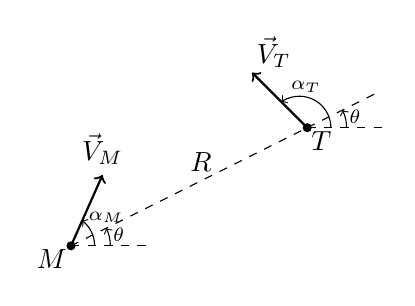
\begin{tikzpicture}

    %% Collision diagram

    % Mass M
    \coordinate (M) at (0,0);
    \draw[fill] (M) circle (0.05) node[below left=-2] {\( M \)};
    \draw[->, thick] (M) -- ++(0.4,0.9) node[above] {\( \vec{V}_M \)};

    % Mass T
    \coordinate (T) at (3,1.5);
    \draw[fill] (T) circle (0.05) node[below right=-2] {\( T \)};
    \draw[->, thick] (T) -- ++(-0.7,0.7) node[above right=-2] {\( \vec{V}_T \)};

    % Line of separation
    \draw[dashed] (M) -- (T) node[pos=0.55, above] {\( R \)};

    % Reference
    \draw[dashed] (M) -- ++(1,0);
    \draw[dashed] (T) -- ++(1,0);
    \draw[dashed] (T) -- ++(0.9,0.45);

    % Angles
    \draw[->] (M) ++(0.5,0) arc (0:27:0.5) node[pos=0.6, right=-2] {\scriptsize \( \theta \)};
    \draw[->] (T) ++(0.5,0) arc (0:27:0.5) node[pos=0.6, right=-2] {\scriptsize \( \theta \)};
    \draw[->] (M) ++(0.3,0) arc (0:54:0.4) node[pos=1.2, right=0.8] {\scriptsize \( \alpha_M \)};
    \draw[->] (T) ++(0.3,0) arc (0:125:0.4) node[above right] {\scriptsize \( \alpha_T \)};

\end{tikzpicture}
\end{document}
